\section{Description of instrumental DetChar}

I did a whole lot of instrumental DetChar.

\section{Tools and algorithms}

\subsection{Omicron}

We use a sine-Gaussian basis to search for excess power

\subsection{Hveto}

One tool that we have often used in Detector Characterization to look 
for time coincidence between glitches (noise transients) in different 
channels is Hveto (Hierarchical Veto). Glitches in each channel are 
identified by external algorithms that have been tuned to search for 
specific patterns in the time series. Any glitch that is reported in 
the output of an external algorithm is referred to as a trigger. 

Typically, Hveto is used to compare a channel that potentially contains 
gravitational wave signals, denoted $h(t)$, and an auxiliary channel 
that does not have direct astrophysical implications. Hveto counts 
the number of coincident triggers between two time series using a 
user-defined time window centered around each trigger in the auxiliary 
channel. The figure of merit returned by Hveto for each auxiliary channel 
after comparison to $h(t)$ is called \textit{significance}.

Significance answers the follow question: how unlikely is it that 
the coincident triggers in these two channels were the result of 
two arbitrary Poisson processes occurring in each channel? 

More specifically, given two arbitrary Poisson processes, how 
unlikely is it that we measure $n$ or more coincident triggers 
given that expected number of coincidences from random chance is $\mu$?

Significance is calculated as (ref Hveto),

\begin{equation}
S = -\log_{10} (\sum\limits_{k = n}^{\infty} P(\mu,k)),
\end{equation}

where $n$ is the number of coincidences found between the two channels 
during the total analysis time and $P(\mu,k)$ is the Poisson probability 
distribution function,
\begin{equation}
P(\mu,k) = \frac{\mu^{k}e^{-\mu}}{k!}.
\end{equation}

Here $\mu$ is the expected number of coincidences between triggers in 
$h(t)$ and the auxiliary channel based solely on chance, which is estimated as,

\begin{equation}
\mu = \frac{N_{h}N_{aux}T_{win}}{T_{tot}},
\end{equation}

where $N_{h}$ and $N_{aux}$ are the number of triggers in $h(t)$ and a 
given auxiliary channel respectively during the total analysis time, 
$T_{tot}$, and $T_{win}$ is the length of the coincidence window used.

A high value of significance indicates that the triggers in the channels 
were very often coincident in time and that there is a very small probability 
that the intersection is a product of random chance. This is a very useful 
measure when we are searching for auxiliary channels that might have some 
noise coupling into our output channel. A significance value of up to 5 is 
often observed in channels with no causal relationship to $h(t)$ (ref Hveto), 
giving us a useful threshold for identifying  effective vetoes.

Another interesting figure of merit used for a given round of Hveto is 
the ratio of $\frac{efficiency}{deadtime}$. Efficiency is defined as the 
percent of triggers vetoed from $h(t)$ during a round of vetoes. Deadtime 
is defined as the percent of total analysis time removed from $h(t)$ during 
a round of vetoes. A ratio of 1 is what we would expect from vetoing time 
at random, indicating no strong time correlation between triggers in the 
two channels. A high value of this ratio, which is ideal, indicates that 
we are vetoing a large number of triggers while maintaining a high percentage 
of our analysis time, indicating that the triggers are often close enough 
in time that we can catch a large number of triggers using a small time window.

When Hveto discovers an auxiliary channel that has a strong correlation 
with $h(t)$, the round winner, it removes all of the time windows surrounding 
auxiliary channel glitches and recalculates the significance of the list of 
auxiliary channels. If a channel's significance has dropped after this removal 
of time, it must have had a large amount of glitches coincident with the 
round winner. The change in significance of each channel is displayed on a 
figure called a `drop-plot`. This is one of the most powerful parts of Hveto
 - the ability to find families of channels that often glitch at the same time.

Ideally, the list of significant channels displayed on the drop-plot will be 
able to localize the issue to a specific subsystem or area of the IFO. 
From there, the issue can be investigated and brought to the attention of 
commissioners for repair or physical inspection. This solution is not possible 
as sometimes the cause of the glitches is unclear, but identifying times of 
poor data quality is still useful.

Using Hveto, we can monitor auxiliary channels to find and remove glitches 
in $h(t)$ that would otherwise pollute a gravitational-wave analysis. Removing 
these glitches serves multiple purposes for the search pipelines. Removing 
high SNR glitches cleans up the background of triggers and allows the search 
pipelines to claim a lower SNR threshold for potential detections. A lower 
SNR threshold implies a larger volume for astrophysical analysis. Removing 
glitches reduces the potential for false alarms in the search pipelines, 
which in turn increases the confidence of eventual detections.


\section{Analog-to-Digital Conversion}

Advanced LIGO interferometers are controlled in real-time using a digital 
control system installed on a series of computers referred to as front end 
computers.  This system overall is referred to as the Front End Control 
(FEC) subsection of the more expansive Control and Data System (CDS).  
In a control loop, the FE computers must be capable of reading in an 
analog signal from the interferometer (position measurements, error signals, 
coil currents, etc), digitally sampling that analog signal, using these now 
digital values in a series of control algorithms, and outputting an analog 
control signal to send back into the interferometer.

The process of digital sampling is handled by an analog-to-digital 
converter (ADC) and the process of analog output is handled by a 
digital-to-analog converter (DAC).  Since these converters are linearly 
mapping a continuous signal onto a discrete range, they are limited by 
their digital bit depth.  For example, a 16 bit ADC is only capable of 
representing $2^{16}$ discrete values, or a range from zero to 65536.  
This range is often centered around zero, giving the ADC the capability 
to handle a range of $\pm32768$.  An incoming analog signal is mapped 
onto this range and converted into a digital signal.

For example, if I was sampling an analog signal with a range of $\pm100V$, 
100V would be mapped to 32768 and -100V would be mapped to -32768 with all 
of the intermediate voltage values being linearly mapped to the range. This 
means our digital system would recognize a discrete step size of 
$100/32768 \approx 3.05 mV$.

Looking at the system described above, we must be aware of how our system 
is going to react when our analog input signal exceeds the intended maximum 
value of 100V (e.g., a 110V input). The ADC has already assigned its maximum 
digital value to 100V. This is called range saturation. In this case the ADC 
will continuously output its maximum value as it has no way to map 110V into 
a discrete value. The same process can occur in a DAC when a digital signal 
is sent out at the maximum allowed digital value.

If the digital system is not able to correctly sample and understand an analog 
error signal, it is easy to imagine a scenario where the reponse of the digital 
system and the output control signal are not able to complete the control loop 
as designed. This may cause glitches or misalignments.

We must also consider the fact that many ADCs are calibrated to reflect the 
intended dynamic range of an optic.  If a saturation is occurring, there is 
a good chance that an optic has moved beyond this intended dynamic range, which 
also may cause glitches or misalignments.

The ADCs and DACs are monitored by a series of auxiliary channels. 
The most useful channels are of the form:

\begin{verbatim}
L1:FEC-21_DAC_OVERFLOW_0_0
\end{verbatim}

Parsing this channel name:

\begin{verbatim}
L1:FEC-{model number}_{ADC/DAC}_OVERFLOW_{ADC/DAC number}_{channel number}
\end{verbatim}

These overflow monitor channels are cumulative. If the channel has no saturation 
at the time of sampling, the overflow channel's reported value will not increase. 
If the channel was saturated during the last sample, the value of the channel will 
increase in discrete steps equal in size to the maximum value of the channel.

Used this to generate flags for veto definer, ETMY driver and OMC DCPD saturations.

\section{Suspension DAC calibration glitches}

We see glitches when suspensions cross values of zero or $2^{16}$.

\textcolor{red}{Discuss Hveto results}

\section{RF beatnote whistles}

Two RF oscillators beating against one another creates a kHz beatnote that couples 
into DARM.

\begin{figure}[ht!]%
\centering
\subfloat[]{
  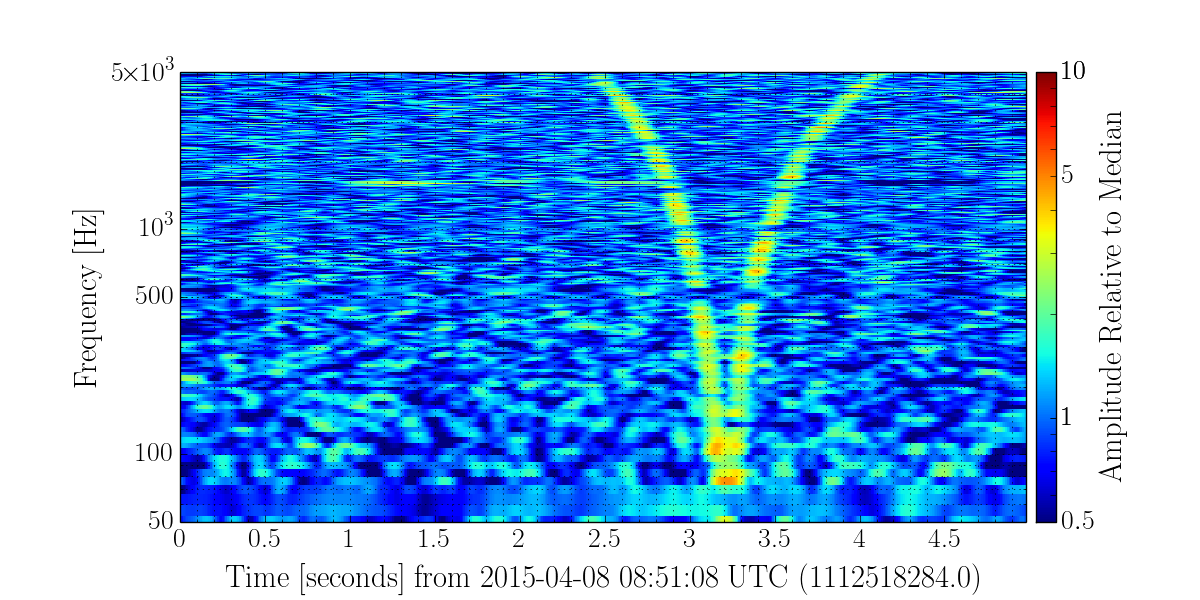
\includegraphics[width=\textwidth]{figures/detchar/Spectrogram_Whistle_LLO}
  \label{subfig:llo-whistle}
  }
  
\subfloat[]{
  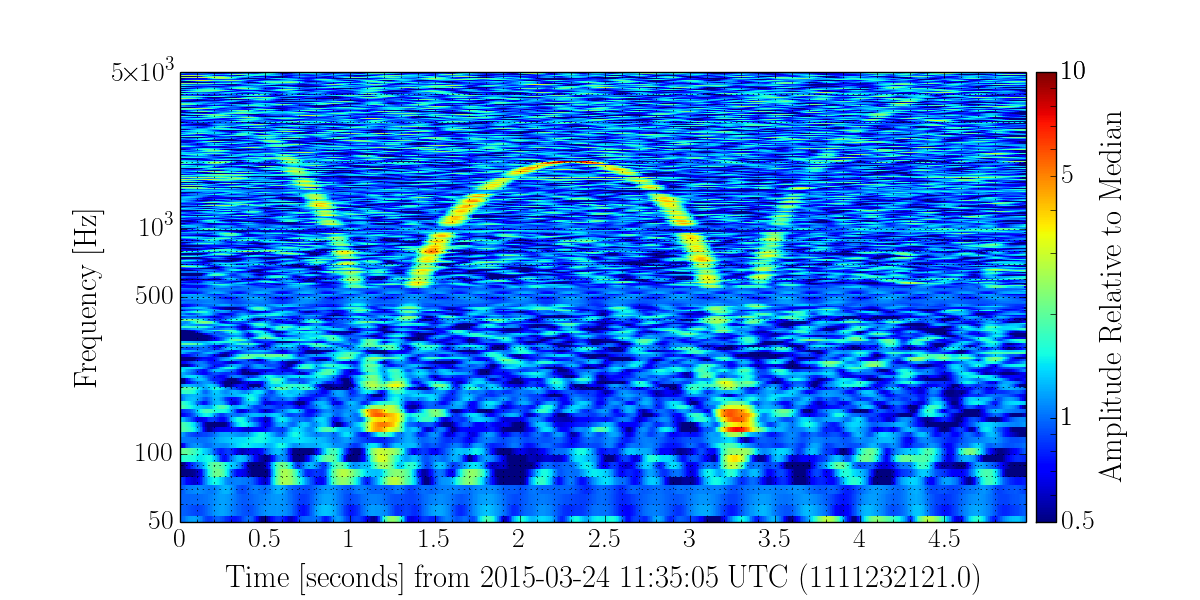
\includegraphics[width=\textwidth]{figures/detchar/Spectrogram_Whistle_LHO}
  \label{subfig:lho-whistle}
  }
\caption[Spectrograms of RF whistles]{Spectrograms of RF whistles at %
         both LLO and LHO. Figure \ref{subfig:llo-whistle} shows a %
         whistle at LLO. Figure \ref{subfig:lho-whistle} shows a whistle %
         at LHO.
         }
\end{figure}\label{fig:whistle-spectrograms}

\section{Seismic CPS comb}

Oscillators in the capacitive position sensors had drifted apart and caused a 
beatnote and a comb. Audio analysis pointed towards amplitude modulation. 

Fixed by slaving all oscillators to a master.

\section{DC values of auxiliary channels}

No great correlation at the end of the day 

\section{Earthquakes during full lock}

Lots of scattering arches during an earthquake, drove up the noise and biased PSD.
Caused a sarlacc, removing this data was able to repair data on either side.

\section{L1 PMC glitches}


Characterization of noise and analysis after repair

\section{Data quality shifts}
Performed and mentored data quality shifts.



